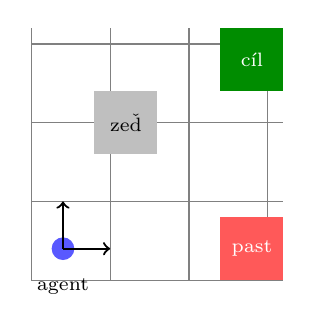
\begin{tikzpicture}[x=0.8cm,y=0.8cm]

    \draw[step=1cm, black!50] (0,0) grid (4,4);

    % překážka
    \fill[black!25] (1,2) rectangle (2,3);
    \node at (1.5,2.5) {\scriptsize zeď};

    % agent
    \fill[blue!65] (0.5,0.5) circle (0.18);
    \node[below, font=\scriptsize] at (0.5,0.18) {agent};

    % cíl
    \fill[green!55!black] (3,3) rectangle (4,4);
    \node[font=\scriptsize, text=white] at (3.5,3.5) {cíl};

    % past
    \fill[red!65] (3,0) rectangle (4,1);
    \node[font=\scriptsize, text=white] at (3.5,0.5) {past};

    % šipky akcí
    \draw[->, thick] (0.5,0.5) -- (1.25,0.5);
    \draw[->, thick] (0.5,0.5) -- (0.5,1.25);

\end{tikzpicture}
